\chapter{Arquitectura general del sistema ALERTAR}\label{cap:arquitecturaGeneral}

El sistema ALERTAR despliega un análisis de triaje automático a partir de la carga de datos provista por el personal de salud, incluyendo signos vitales, comorbilidades, resultados de laboratorio e informes radiográficos. La clasificación de los pacientes se realiza en cuatro niveles de gravedad, basados en la proyección de su evolución en las próximas 24 o 48 horas: bajo, moderado, alto y crítico, este último requiriendo atención en la unidad de cuidados intensivos. En caso de que se produzca un cambio en la gravedad, el sistema envía alertas al personal de salud, al mismo tiempo que organiza y coordina sus tareas con un enfoque de atención centrado en el paciente.

En la sección \ref{sec:componentesSistema} se explican los componentes que conforman el sistema y la función que cumplen dentro de este. En la sección \ref{sec:OrganizacionYUbicacionDatos} se explica cómo están organizados y ubicados los datos en función de la resiliencia.
%Diapo 5
\section{Componentes del sistema}
\label{sec:componentesSistema}
La diversidad en la calidad y estabilidad de las conexiones a Internet en los hospitales de Argentina es un factor de suma importancia. En este contexto, aún en casos de inestabilidad de la conectividad con el mundo exterior, el sistema debe permitir que:
\begin{itemize}
    \item El personal de la salud cuente con la capacidad de ingresar datos de los pacientes desde la sala en la que están asignados.
    \item Se emitan alertas tempranas en cualquier momento.
    \item Se preserve la coherencia e integridad de los datos.
\end{itemize}

El sistema no debe estar sujeto a la dependencia de un servidor estándar dentro de los hospitales. Esto se fundamenta en la necesidad de simplificar tanto la implementación como el mantenimiento del sistema, evitando así la complejidad adicional que podría surgir de la gestión de servidores locales.

Por otro lado, para potenciar el análisis de datos y el descubrimiento de nuevos conocimientos, es esencial contar con un repositorio global e histórico de datos. Esta fuente de información permitirá la generación de estadísticas relevantes y la extracción de nuevos conocimientos que contribuyan al avance y mejora de la atención médica en general \cite{canibano2022towards}.

En pos de todo esto, la arquitectura del sistema se resume en tres niveles computacionales los cuales se pueden observar en la Figura \ref{fig:arqGeneral}:\\

\begin{figure}
    \centering
    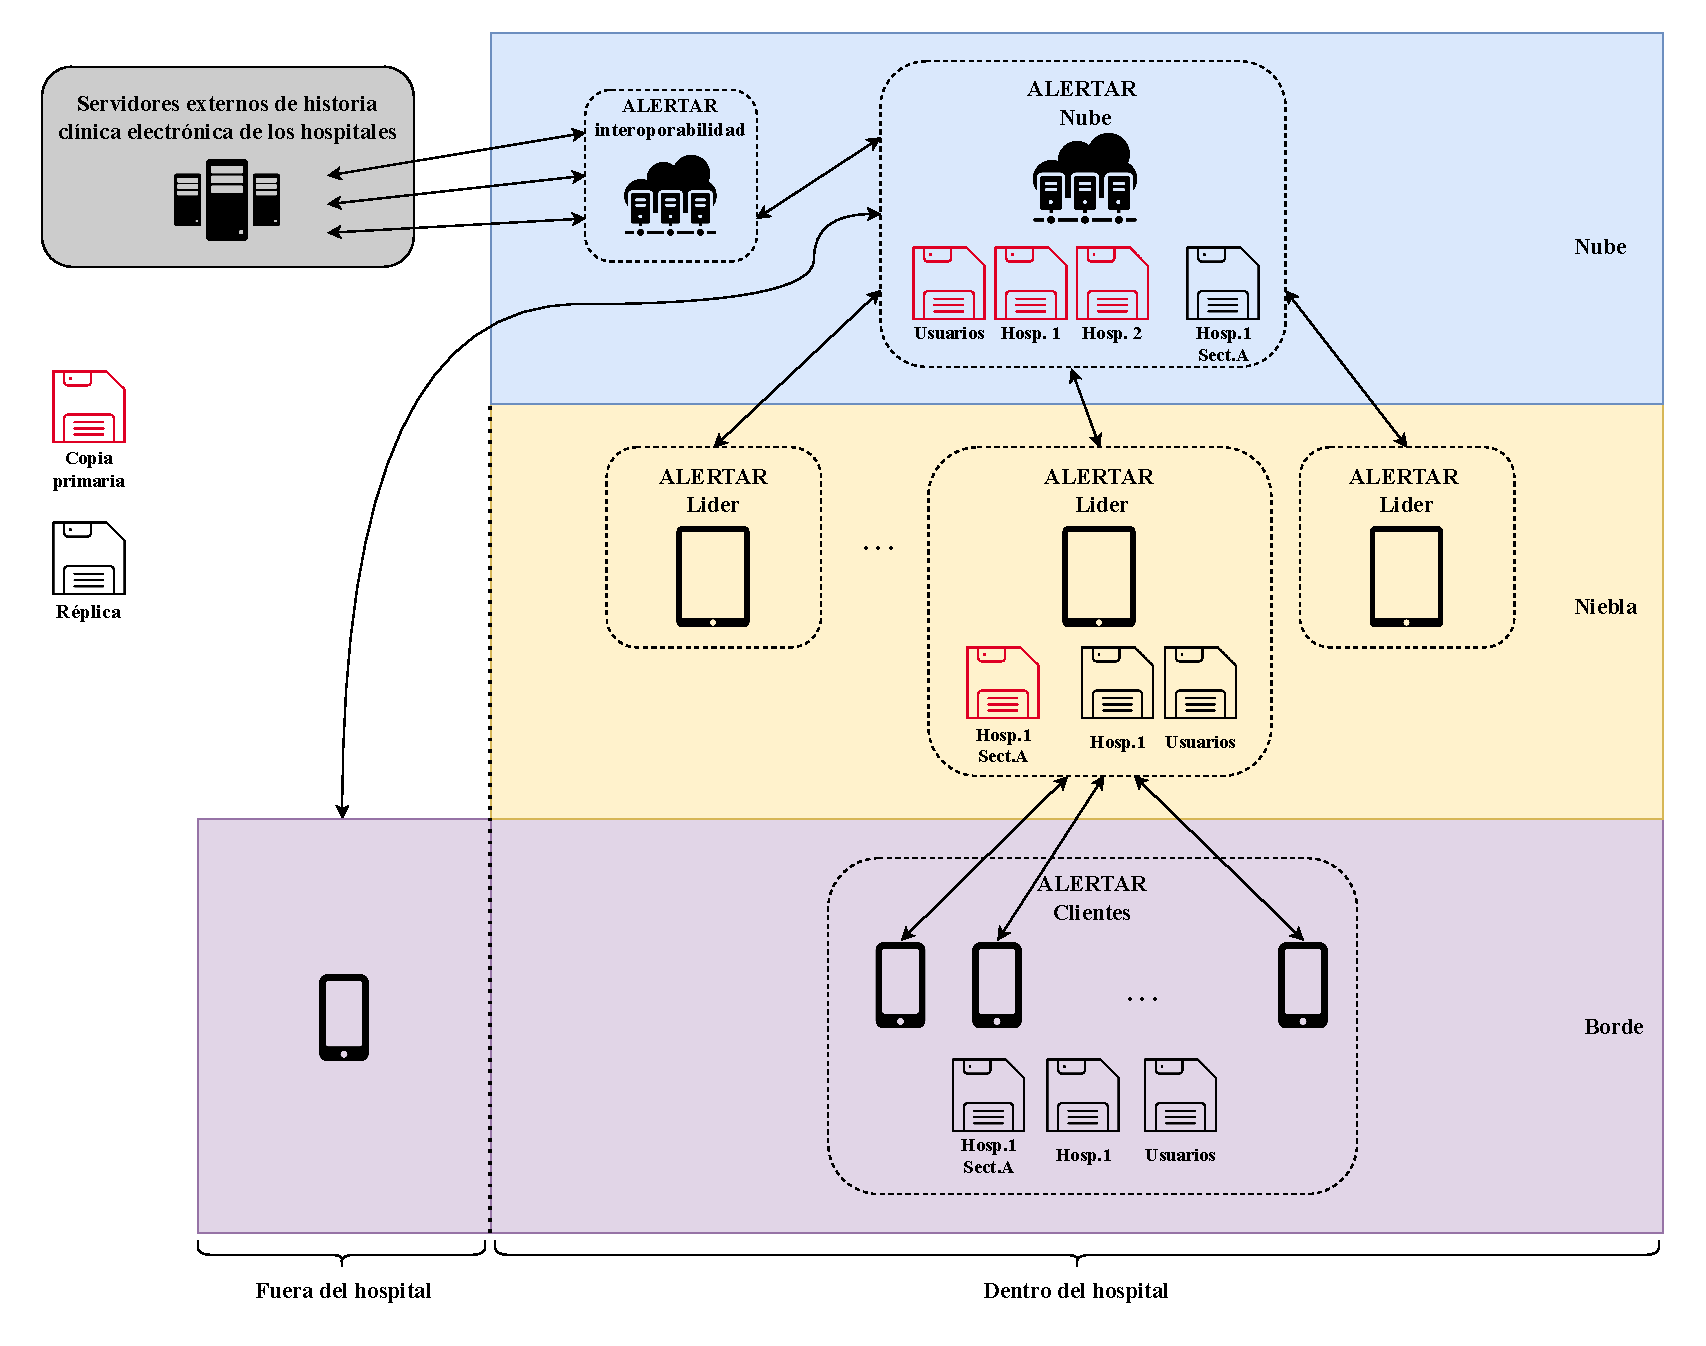
\includegraphics[width=\textwidth]{Imagenes/Arquitectura General/Componentes del sistema.pdf}
    \caption{Arquitectura de ALERTAR}
    \label{fig:arqGeneral}
\end{figure}
\textbf{Borde \textit{(Edge)}:} El término ``Dispositivo de borde'' se refiere a los dispositivos móviles empleados por el personal médico y de enfermería. Estos dispositivos posibilitan el ingreso de datos del sistema y la observación de resultados. Establecen una conexión directa con el nivel de niebla en caso de encontrarse en la misma red de área local, o con el nivel de la nube mediante Internet. Siempre priorizando la conexión con la capa de niebla.\\


\textbf{Niebla \textit{(Fog)} :} Se refiere a dispositivos móviles ubicados dentro del hospital. Estos atienden a los dispositivos de borde a través de una conexión de red de área local. La conexión a nivel niebla permite que los hospitales en entornos donde el acceso a Internet puede ser limitado, debido a restricciones de costo o a una conexión intermitente, puedan trabajar de manera efectiva y sin interrupciones.\\

\textbf{Nube \textit{(Cloud)}:} La nube mantiene una copia exhaustiva e histórica de todas las bases de datos de dispositivos a nivel de niebla. Además de ser la principal reserva de datos administrativos del hospital, almacena información compartida entre todos los hospitales. Esta capacidad de almacenamiento centralizado simplifica la gestión y el acceso a la información para todos los usuarios autorizados. Por otro lado, la conexión a nivel de la nube, actúa como nexo entre los dispositivos que se encuentren fuera de los hospitales y la capa de niebla.

%Usar orden de las diapos THAIS_2023
%Datos en reposo
\section{Organización y ubicación de los datos}
\label{sec:OrganizacionYUbicacionDatos}

El almacenamiento de datos se organiza en función de la resiliencia. Es decir que el lugar donde se almacenan los datos y de qué manera se hace, se determina en función de los servicios que tengan la capacidad de mantenerse operativos, de manera completa o parcial, ante la ocurrencia de fallos. El almacenamiento se organiza en copias primarias y réplicas. Las copias primarias son la copia original de los datos. Las réplicas son duplicados exactos utilizados para tener tolerancia a fallos.


El dominio de datos se divide en los siguientes dominios:
\begin{itemize}
    \item \textbf{Dominio de usuarios:} Contiene los datos personales del personal de salud que trabaja en los hospitales, como nombres, direcciones de correo electrónico y datos de contraseñas. Solo existe una instancia de este dominio. La nube posee la copia primaria de este dominio. Los dispositivos de niebla y borde poseen réplicas de este dominio.
    \item \textbf{Dominios de hospitales:} Comprende la información específica de cada hospital, como su nombre, dirección y otros detalles relevantes. Además, incluye datos sobre los usuarios que forman parte del personal del hospital, como su número de identificación y rol en la institución. También se encuentran registros relacionados con los diferentes sectores o áreas funcionales dentro del hospital. Cada hospital tiene su propia instancia de dominio, lo que permite una gestión detallada y personalizada de la información para cada centro médico. La nube posee la copia primaria de estos dominios. Los dispositivos de niebla y borde poseen réplicas del dominio hospital en el que se encuentran.
    \item \textbf{Dominios de sectores:} Contiene la información de cada área funcional o sector dentro del hospital. Esto incluye información de alertas médicas, datos personales y clínicos de los pacientes, información sobre la disponibilidad de camas y personal asignado al sector. Además, se registran eventos importantes como la apertura y el cierre de episodios clínicos, junto con los procesos de ingreso y egreso de pacientes. Un dispositivo de niebla es asignado para ``liderar'' a cada sector, este dispositivo es el que contiene la copia primaria del sector. El dispositivo a cargo del sector puede cambiar en cualquier momento y su reemplazo pasará a tener la copia primaria. Los dispositivos de borde poseen réplicas del dominio del sector en el que se encuentran y la nube posee réplicas de todos los dominios sector.
    
\end{itemize}
 Cada instancia de dominio es asociada con un componente del sistema, dispositivo de niebla o nube, que mantiene la copia primaria de los datos. Cuando un dispositivo desea almacenar un registro de datos para un dominio específico, debe enviar una solicitud al componente del sistema que posee la copia primaria de ese dominio. Una vez que el dato fue exitosamente almacenado en la copia primaria, se envía una copia a todos los dispositivos de borde de ese dominio, incluido el dispositivo que realizó la solicitud. 
 
 Además, el dispositivo que contiene la copia primaria de un dominio, puede procesar los nuevos registros en conjunto con los datos históricos a fin de generar nuevos registros. Por ejemplo, la inserción de un nuevo registro de paciente puede generar un nuevo registro relacionado con la clasificación de triaje.
 
 En la Figura \ref{fig:arqGeneral} se observan las copias primarias y réplicas de los tres tipos de dominios. Ante la ocurrencia de fallos, componentes del sistema que mantengan réplicas suplantarán, completa o parcialmente, la funcionalidad de los componentes que mantenían las copias primarias.

 Para permitir la sincronización de las réplicas, cada dominio cuenta con un reloj lógico que se incrementa al momento de la inserción de cada nuevo dato. Cada dato insertado va acompañado del nuevo valor del reloj.





